\documentclass[conference]{IEEEtran}
\usepackage[utf8]{inputenc}
\usepackage{graphicx}
\usepackage{booktabs}
\usepackage{amsmath}
\usepackage{hyperref}
\usepackage{iftex}
\ifXeTeX
  \usepackage{fontspec}
  \setmainfont{texgyretermes}[Extension=.otf,UprightFont=*-regular,BoldFont=*-bold,ItalicFont=*-italic,BoldItalicFont=*-bolditalic]
\fi

\title{RAG and Agentic RAG for Financial Questions over SEC Filings: An Ablation Study of Five Architectures with Validated \textit{Ground Truth}}

\author{
\IEEEauthorblockN{Fernando José Soto Jácome}
\IEEEauthorblockA{Universidad San Francisco de Quito (USFQ) \\
fsotoj@estud.usfq.edu.ec}
}

\begin{document}

\maketitle

\begin{abstract}
This work evaluates how much each component of a \textit{Retrieval-Augmented Generation} (RAG) system contributes to the quality of financial answers, and at what cost. Over a corpus of 206 10-K and 10-Q filings of 10 Nasdaq-100 companies (6{,}536 \textit{chunks}, $\sim$6M words), five systems of increasing complexity were built: BM25, vector search (BGE-M3 + FAISS), hybrid fusion (RRF), hybrid with a \textit{knowledge graph}, and a ReAct agent in LangGraph with search, calculation and XBRL data tools. The systems were evaluated on 35 questions of seven types, whose expected answers were validated against the corpus by independent LLM judges. With the three RAGAS metrics, the agent obtained the highest \textit{answer correctness} (0.441 versus 0.373 for the best vector baseline and 0.334 for BM25), but the lowest \textit{faithfulness} (0.429 versus 0.930), using 3.8 LLM calls and 3.2 times more latency per query with a similar token volume ($\sim$16k). Hybrid fusion and the \textit{knowledge graph} improved retrieval (\textit{context recall} from 0.346 to 0.458), but not the final answer. No system exceeded 45\% \textit{answer correctness}, which indicates that, in this domain, the bottleneck is retrieving the right evidence and not only reasoning over it.
\end{abstract}

\begin{IEEEkeywords}
RAG, Agentic RAG, LangGraph, RAGAS, knowledge graph, financial questions, natural language processing
\end{IEEEkeywords}

\section{Introduction and Related Work}

RAG \cite{lewis2020rag} combines a document retriever with a generative language model so that answers rely on external evidence and not only on the parametric knowledge of the model. In the financial domain this property is critical: an analyst needs exact figures, with their correct fiscal period and traceable to the source document. The SEC 10-K and 10-Q filings hold that information, but they are documents of more than one hundred pages that mix tables, narrative text and fiscal periods that do not match the calendar year.

Retrieval in RAG has been approached lexically, with BM25 \cite{robertson2009bm25}; densely, with multilingual \textit{embeddings} such as BGE-M3 \cite{chen2024bgem3} indexed in FAISS \cite{johnson2019faiss}; or by combining both lists through \textit{Reciprocal Rank Fusion} (RRF) \cite{cormack2009rrf}. More recent proposals add a \textit{knowledge graph} built with LLMs over the corpus (GraphRAG \cite{edge2024graphrag}) or turn the system into an agent that interleaves reasoning and tool use (ReAct \cite{yao2023react}). Each component adds complexity and cost, but its individual contribution is rarely measured on the same set of questions.

For evaluation, RAGAS \cite{es2024ragas} proposes LLM-judge-based metrics that separate retrieval quality (\textit{context recall}) from generation quality (\textit{faithfulness}, \textit{answer correctness}). Two of these metrics depend on a reference answer; if that reference is wrong, so is the metric. Using LLMs as judges \cite{zheng2023judge} makes it possible to validate those references at scale, although with their own biases. On financial questions, FinQA \cite{chen2021finqa} showed that numerical reasoning over filings is hard even when the evidence is available.

This work carries out an \textit{ablation study} of five RAG architectures over SEC filings, with a \textit{ground truth} validated by LLM judges and an explicit comparison of quality and cost.

\section{Methodology}

\subsection{Corpus}
The 10-K and 10-Q filings of the 10 largest companies by weight in the Nasdaq-100 (NVDA, AAPL, MSFT, GOOGL, MU, AMZN, AMD, META, TSLA, AVGO) were downloaded from SEC EDGAR for fiscal years 2020--2026, for a total of 206 documents. Each HTML file was normalized to text by section (Item 1, Item 7, etc.), keeping the company, form type and period end date as metadata. The text was segmented with a paragraph-aware splitter with overlap into 6{,}536 \textit{chunks} (median of 319 words, $\sim$6M words in total), each with a \texttt{[Company | Document | Section]} header that the LLM can cite.

\subsection{Evaluated Systems}
The five systems share the corpus and differ in one component at a time (Table~\ref{tab:sistemas}):

\begin{itemize}
\item \textbf{S1 BM25} (lexical baseline): Okapi BM25, top-8 \textit{chunks}, one LLM call.
\item \textbf{S2 Vector} (semantic baseline): 1024-dimensional BGE-M3 \textit{embeddings} generated on an H200 GPU and cosine search in FAISS (\texttt{IndexFlatIP}), top-8.
\item \textbf{S3 Hybrid}: fusion of the S1 and S2 lists with RRF ($k=60$), top-8.
\item \textbf{S4 Hybrid+KG}: S3 plus a subgraph of a \textit{knowledge graph} (943 nodes, 1{,}477 edges) built by extracting entities and relations with gpt-4o-mini. 5 entities and 5 relations are added to the prompt, and the \textit{chunks} are truncated to 1000 characters.
\item \textbf{S5 Agentic} (proposed solution): ReAct agent in LangGraph with three tools: \texttt{search} (hybrid + KG, top-15), \texttt{get\_financial\_facts} (structured SEC XBRL data) and \texttt{calculator}. A memory node records the failed tools and the searches already done, and a limit of 3 iterations forces a final answer.
\end{itemize}

\textbf{Use of each LLM.} gpt-4o-mini (temperature 0) generates the answers of S1--S4 and extracted the entities and relations of the \textit{knowledge graph}. GLM-5.3-Flash, served on a self-hosted endpoint, generates the answers of S5 and acts as the RAGAS judge.

\begin{table}[h]
\centering
\footnotesize
\setlength{\tabcolsep}{3pt}
\begin{tabular}{lllc}
\toprule
\textbf{System} & \textbf{Retrieval} & \textbf{\textit{Chunks} to the LLM} & \textbf{Calls} \\
\midrule
S1 BM25 & BM25 & 8 full & 1 \\
S2 Vector & BGE-M3 + FAISS & 8 full & 1 \\
S3 Hybrid & S1 + S2 with RRF & 8 full & 1 \\
S4 Hybrid+KG & S3 + KG subgraph & 8 (1000 char.) + KG & 1 \\
S5 Agentic & Agent + 3 \textit{tools} & 15 (800 char.)/search & 1--4 \\
\bottomrule
\end{tabular}
\caption{Systems of the ablation study.}
\label{tab:sistemas}
\end{table}

\subsection{Evaluation Set}
The evaluation uses 35 questions of seven types (Table~\ref{tab:preguntas}). Five types have a concrete expected answer: single figures, comparisons across companies, calculations over several figures, \textit{multi-hop} questions that combine several sections of a filing, and explanations of a company's strategy. The other two are adversarial and their correct answer is not a number: in the ambiguous questions the year, period or metric type is missing, and the system is expected to ask for clarification; in the knowledge-gap ones the information is not in the 10-K/10-Q filings, and the system is expected to admit it.

\begin{table*}[t]
\centering
\small
\begin{tabular}{lcl}
\toprule
\textbf{Type} & \textbf{Questions} & \textbf{Example} \\
\midrule
Numeric & 7 & \textit{What was Apple's total revenue in fiscal year 2023?} \\
Comparative & 4 & \textit{Between Google and Amazon, which had better operating margin in 2023?} \\
Calculation & 5 & \textit{What was Amazon's operating cash flow as a percentage of revenue in 2023?} \\
\textit{Multi-hop} & 6 & \textit{How did NVIDIA's acquisition strategy relate to their AI business growth in 2023?} \\
Explanatory & 5 & \textit{Why did Apple's revenue decline in fiscal 2023 despite strong brand performance?} \\
Ambiguity & 5 & \textit{How much did Tesla spend on capital expenditures?} \\
Knowledge gap & 3 & \textit{What is the current stock price of Tesla?} \\
\midrule
\textbf{Total} & \textbf{35} & \\
\bottomrule
\end{tabular}
\caption{Distribution of the 35 evaluation questions with an example of each type.}
\label{tab:preguntas}
\end{table*}

The expected answers were validated against the corpus by LLM judges working blindly, without knowing each other's verdicts. GPT-6 Astra validated the 35 questions. Claude Opus 5.5 independently reviewed 16 of them (the 6 with figures that needed additional verification and the 10 adversarial ones), agreeing on 15 of 16. In the only disagreement, the answer with evidence in the corpus was kept.

\subsection{Metrics}
Three RAGAS metrics were used, with BGE-M3 for the \textit{embeddings}: \textit{faithfulness} (the answer is supported by the retrieved \textit{contexts}), \textit{context recall} (the \textit{contexts} contain the information of the expected answer) and \textit{answer correctness} (factual and semantic similarity to the expected answer), the latter as the main accuracy measure. Cost is measured in tokens per query, LLM calls, latency and USD at the gpt-4o-mini price (\$0.15 per million input tokens and \$0.60 per million output tokens).

\section{Results and Discussion}
\label{sec:resultados}

\subsection{Quality: RAGAS Metrics}
Table~\ref{tab:ragas} and Figure~\ref{fig:ragas} show the three metrics per system over the 35 validated questions. No architecture dominates in all three: S2 has the highest \textit{faithfulness}, S4 the highest \textit{context recall} and S5 the highest \textit{answer correctness}.

\begin{table}[h]
\centering
\small
\begin{tabular}{lccc}
\toprule
\textbf{System} & \textbf{Faithf.} & \textbf{Ctx. recall} & \textbf{Ans. corr.} \\
\midrule
S1 BM25      & 0.901 & 0.322 & 0.334 \\
S2 Vector    & \textbf{0.930} & 0.346 & 0.373 \\
S3 Hybrid    & 0.863 & 0.398 & 0.295 \\
S4 Hybrid+KG & 0.762 & \textbf{0.458} & 0.312 \\
S5 Agentic   & 0.429 & 0.199 & \textbf{0.441} \\
\bottomrule
\end{tabular}
\caption{RAGAS metrics per system (35 validated questions). The best value of each metric is in bold.}
\label{tab:ragas}
\end{table}

\begin{figure}[h]
\centering
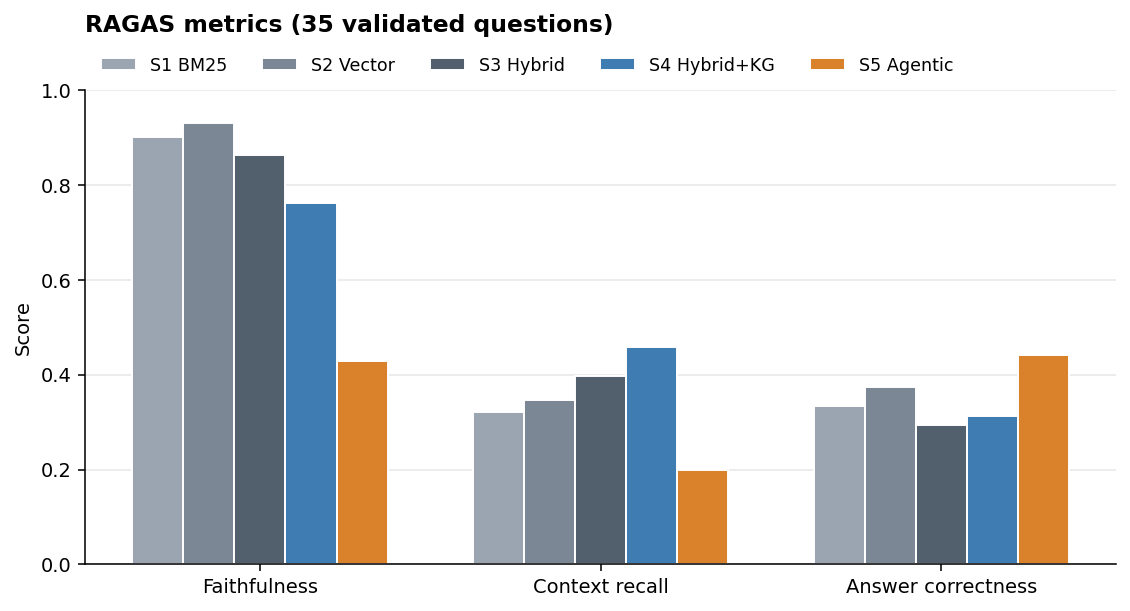
\includegraphics[width=\linewidth]{fig_ragas.png}
\caption{RAGAS metrics per system.}
\label{fig:ragas}
\end{figure}

\subsection{Ablation: Contribution of Each Component}
Table~\ref{tab:ablacion} isolates the effect of adding each component.

\begin{table}[h]
\centering
\small
\begin{tabular}{lccc}
\toprule
\textbf{Step} & \textbf{$\Delta$Faithf.} & \textbf{$\Delta$Recall} & \textbf{$\Delta$Corr.} \\
\midrule
BM25 $\rightarrow$ Vector      & +2.9  & +2.4  & +3.9 \\
Vector $\rightarrow$ Hybrid    & $-$6.8  & +5.2  & $-$7.8 \\
Hybrid $\rightarrow$ +KG       & $-$10.1 & +6.0  & +1.7 \\
+KG $\rightarrow$ Agent        & $-$33.3 & $-$25.9 & +12.9 \\
\midrule
BM25 $\rightarrow$ Agent       & $-$47.2 & $-$12.3 & +10.7 \\
\bottomrule
\end{tabular}
\caption{Differences in percentage points when adding each component. The last row compares the baseline (S1) with the solution (S5).}
\label{tab:ablacion}
\end{table}

\textbf{Semantic versus lexical search.} S2 improves on S1 in all three metrics. BM25 rewards long \textit{chunks} with many repetitions of the query terms: in 3 of the 35 questions it retrieved whole sections that the \textit{chunker} did not split (e.g., the entire Item 8 of Amazon's 10-K, with more than 100{,}000 characters). The prompt exceeded the 128k-token window of gpt-4o-mini and the query was rejected without an answer.

\textbf{More retrieval does not imply better answers.} Hybrid fusion and the \textit{knowledge graph} increase \textit{context recall} by 11.2 points over S2, but \textit{answer correctness} drops from 0.373 to 0.295 and 0.312. More relevant \textit{contexts}, mixed with more noise, do not help the LLM pick the correct figure. S4, moreover, changes two things with respect to S3: it adds the subgraph (about 120 tokens with 5 entities and 5 relations) and cuts each \textit{chunk} to 1000 characters before sending it to the LLM, while S1--S3 send the full \textit{chunk}. That cut leaves financial tables incomplete and is the most likely explanation for the 10.1-point drop in \textit{faithfulness}; therefore, the difference between S3 and S4 cannot be attributed to the graph alone.

\textbf{The agent answers better, but RAGAS cannot verify it.} S5 obtains the highest \textit{answer correctness} (+6.8 points over S2 and +10.7 over S1). Its advantage shows up in calculation questions: on Amazon's operating cash flow as a percentage of its revenue, the agent retrieves both values and performs the division, while S1 does not answer and S4 states that it does not have enough information. Its \textit{faithfulness} (0.429) and \textit{context recall} (0.199), in contrast, are the lowest. This is largely explained by the way it is evaluated: the outputs of \texttt{get\_financial\_facts} and \texttt{calculator} are not part of the \textit{contexts} that RAGAS evaluates, and \texttt{search} returns previews of 800 characters. RAGAS then marks as unsupported claims that do come from a tool.

\subsection{Cost}
Table~\ref{tab:costos} compares the cost per query over the 31 questions that the five systems answered. The total project spend on gpt-4o-mini was approximately USD 6, including the knowledge graph extraction (USD 0.22). S5 and the RAGAS judge ran on the self-hosted GLM endpoint at no monetary cost; for comparison, their token usage is valued at the same gpt-4o-mini price.

\begin{table}[h]
\centering
\small
\begin{tabular}{lcccc}
\toprule
\textbf{System} & \textbf{Tokens} & \textbf{Calls} & \textbf{Lat. (s)} & \textbf{USD/1k} \\
\midrule
S1 BM25      & 17{,}121 & 1.00 & 3.5 & 2.61 \\
S2 Vector    & 15{,}064 & 1.00 & 2.6 & 2.30 \\
S3 Hybrid    & 16{,}463 & 1.00 & 3.2 & 2.51 \\
S4 Hybrid+KG & \textbf{2{,}388} & 1.00 & 8.6 & \textbf{0.52} \\
S5 Agentic   & 16{,}251 & 3.84 & 8.3 & 2.64 \\
\bottomrule
\end{tabular}
\caption{Mean cost per query (31 common questions). Tokens computed over the prompts sent to the LLM; USD per 1000 queries at the gpt-4o-mini price.}
\label{tab:costos}
\end{table}

The agent does not consume more tokens than the single-step baselines: its searches return short previews that offset the history accumulated between calls. Its real cost is in the number of calls (3.84 per query) and in latency, 3.2 times that of S2. S4 is the cheapest system, with about 7 times fewer tokens than the rest. This is due to cutting each \textit{chunk} to 1000 characters and not to the graph, which only adds about 120 tokens. Figure~\ref{fig:tradeoff} summarizes the relation between quality and cost: S5 is the only system that clearly improves \textit{answer correctness}, at a token cost equivalent to that of S1--S3.

\begin{figure}[h]
\centering
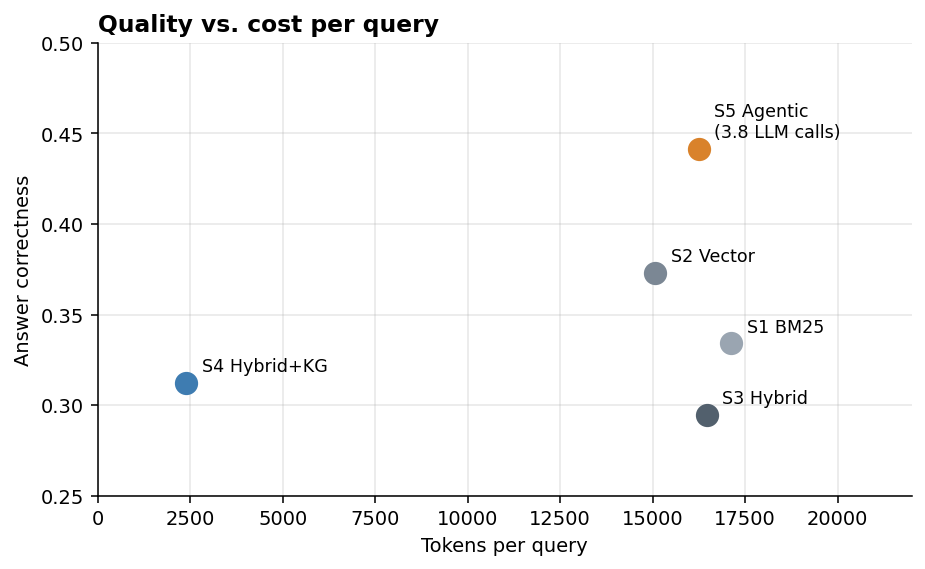
\includegraphics[width=0.95\linewidth]{fig_tradeoff.png}
\caption{\textit{Answer correctness} versus tokens per query.}
\label{fig:tradeoff}
\end{figure}

\subsection{Adversarial Questions}
On the 8 questions whose correct answer is to ask for clarification or to admit ignorance, we counted, with a single text rule, whether each system pointed out the ambiguity or the limit of the information (Table~\ref{tab:adversarial}). S4 did so in all 8, and S2 in 7. The agent did so in 4 and recognized only 1 of the 3 knowledge gaps: when a tool does not find the information, it tends to build an answer with what it did find instead of stating the absence.

\begin{table}[h]
\centering
\small
\begin{tabular}{lccc}
\toprule
\textbf{System} & \textbf{Ambiguity (5)} & \textbf{Gap (3)} & \textbf{Total (8)} \\
\midrule
S1 BM25      & 2 & 3 & 5 \\
S2 Vector    & 4 & 3 & 7 \\
S3 Hybrid    & 2 & 3 & 5 \\
S4 Hybrid+KG & \textbf{5} & \textbf{3} & \textbf{8} \\
S5 Agentic   & 3 & 1 & 4 \\
\bottomrule
\end{tabular}
\caption{Answers that point out the ambiguity or the lack of information.}
\label{tab:adversarial}
\end{table}

\section{Conclusions}

None of the added components improved retrieval and the answer at the same time. Semantic search was the only consistent improvement over the lexical baseline. Hybrid fusion and the \textit{knowledge graph} retrieve more evidence, but do not turn it into better answers. The agent with tools is the only architecture that clearly increases \textit{answer correctness} (0.441), with a token volume similar to the single-step systems, but with almost four LLM calls, three times more latency, a \textit{faithfulness} evaluation that does not capture the evidence of its tools, and less willingness to admit that it does not know. With a maximum of 44\% \textit{answer correctness}, no system is reliable for financial analysis without supervision.

\textbf{Limitations.} The sample is small (35 questions, 31 in the cost comparison) and no significance tests were applied, so differences of a few points may be due to chance. S5 uses a different LLM from S1--S4, so its advantage cannot be attributed only to the agentic architecture. Both the RAGAS judge and the validation of the \textit{ground truth} are LLMs, not human analysts. S4 adds the graph and at the same time cuts the \textit{chunks}, so its effect is not attributable to the \textit{knowledge graph} alone. The adversarial behavior was measured with a text rule, and the corpus is limited to 10 companies, to 2020--2026 and to 10-K/10-Q filings.

\textbf{Future work.} Evaluate the five systems with the same LLM to isolate the effect of the architecture; include the outputs of all the agent's tools in the \textit{contexts} evaluated by RAGAS; impose a maximum size on the \textit{chunks}, whose absence caused the BM25 overflows; extend the validated set with a human analyst's review; and add to the agent an explicit abstention rule for when its tools do not find the information.

\begin{thebibliography}{10}
\small
\setlength{\itemsep}{0pt}
\bibitem{lewis2020rag} P. Lewis, E. Perez, A. Piktus, F. Petroni, V. Karpukhin, N. Goyal, H. Küttler, M. Lewis, W. Yih, T. Rocktäschel, S. Riedel, D. Kiela, ``Retrieval-Augmented Generation for Knowledge-Intensive NLP Tasks,'' \textit{Proc. NeurIPS}, 2020.
\bibitem{robertson2009bm25} S. Robertson, H. Zaragoza, ``The Probabilistic Relevance Framework: BM25 and Beyond,'' \textit{Foundations and Trends in Information Retrieval}, vol. 3, no. 4, 2009.
\bibitem{chen2024bgem3} J. Chen, S. Xiao, P. Zhang, K. Luo, D. Lian, Z. Liu, ``BGE M3-Embedding: Multi-Lingual, Multi-Functionality, Multi-Granularity Text Embeddings Through Self-Knowledge Distillation,'' \textit{Findings of ACL}, 2024.
\bibitem{johnson2019faiss} J. Johnson, M. Douze, H. Jégou, ``Billion-Scale Similarity Search with GPUs,'' \textit{IEEE Trans. Big Data}, vol. 7, no. 3, 2021.
\bibitem{cormack2009rrf} G. V. Cormack, C. L. A. Clarke, S. Büttcher, ``Reciprocal Rank Fusion Outperforms Condorcet and Individual Rank Learning Methods,'' \textit{Proc. SIGIR}, 2009.
\bibitem{edge2024graphrag} D. Edge, H. Trinh, N. Cheng, J. Bradley, A. Chao, A. Mody, S. Truitt, J. Larson, ``From Local to Global: A Graph RAG Approach to Query-Focused Summarization,'' \textit{arXiv:2404.16130}, 2024.
\bibitem{yao2023react} S. Yao, J. Zhao, D. Yu, N. Du, I. Shafran, K. Narasimhan, Y. Cao, ``ReAct: Synergizing Reasoning and Acting in Language Models,'' \textit{Proc. ICLR}, 2023.
\bibitem{es2024ragas} S. Es, J. James, L. Espinosa-Anke, S. Schockaert, ``RAGAS: Automated Evaluation of Retrieval Augmented Generation,'' \textit{Proc. EACL (System Demonstrations)}, 2024.
\bibitem{zheng2023judge} L. Zheng, W.-L. Chiang, Y. Sheng, S. Zhuang, Z. Wu, Y. Zhuang, Z. Lin, Z. Li, D. Li, E. Xing, H. Zhang, J. E. Gonzalez, I. Stoica, ``Judging LLM-as-a-Judge with MT-Bench and Chatbot Arena,'' \textit{Proc. NeurIPS Datasets and Benchmarks}, 2023.
\bibitem{chen2021finqa} Z. Chen, W. Chen, C. Smiley, S. Shah, I. Borova, D. Langdon, R. Moussa, M. Beane, T.-H. Huang, B. Routledge, W. Y. Wang, ``FinQA: A Dataset of Numerical Reasoning over Financial Data,'' \textit{Proc. EMNLP}, 2021.
\end{thebibliography}

\end{document}
